% \documentclass{article}
\documentclass[fleqn]{article}

\usepackage{notations}
\usepackage{amsfonts}
\usepackage{amsmath}
\usepackage{relsize}
\usepackage{geometry}


\geometry{
 a4paper,
 total={170mm,257mm},
 left=20mm,
 top=20mm,
 }

% ======================================================================================================================
% COMMANDS
% ======================================================================================================================

% \newcommand{\Hbroken}{
%   H^1(\Mesh; \mathbb{R}^{d})
% }

% ======================================================================================================================
% NOTATIONS
% ======================================================================================================================

% \setlength{\mathindent}{0pt}
\setlength{\parindent}{0em}
\setlength{\parskip}{1em}
\renewcommand{\baselinestretch}{1.0}

\title{Introduction to the HHO method}
\author{David Siedel \and Olivier Fandeur \and  Thomas Helfer}

\date{01/08/2020}




% ======================================================================================================================
% DOCUMENT
% ======================================================================================================================

\begin{document}

  \maketitle

%   \section{Notations}

%     \begin{itemize}
%       \item $a$ denotes a scalar value, usually a parameter, a real number, etc.
%       \item $\tensoro{a}$ denotes a $0$-th order tensor-valued function.
%       \item $\tensori{a} = \begin{pmatrix}
%         \tensoro{a}_1 \\ \vdots \\ \tensoro{a}_n
%       \end{pmatrix}$ denotes a $1$-st order tensor-valued function.
%       \item $\tensorii{a} = \begin{pmatrix}
%         \tensoro{a}_{11} & \dots & \tensoro{a}_{1n} \\ \vdots & \ddots & \vdots \\ \tensoro{a}_{N1} & \dots & \tensoro{a}_{Nn}
%       \end{pmatrix}$ denotes a $2$-nd order tensor-valued function.
%       \item $\tensoriv{a}$ denotes a $4$-th order tensor-valued function.
%       \item $\tensorii{a}^t$ denotes the transpose of $\tensorii{a}$
%     \end{itemize}

    % \newpage
    
  \section{Model problem}

        Let a solid $\Omega$. It morphs through the action of volumetric forces in its inner body, and through the influence of contacts forces and imposed displacements at its surface.
        \par

        Let $\partial \Omega = \partial \Omega_N \oplus \partial \Omega_D$ with $\partial \Omega_N \subset \partial \Omega$ the boundary of the body subjected to contact forces (\textit{i.e.} subjected to Neumann boundary conditions), and $\partial \Omega_D \subset \partial \Omega$ the boundary of the body subjected to imposed displacements (\textit{i.e.} subjected to Dirichlet boundary conditions).
        \par

        Let $\tensori{t}\subscript{N}$ contact forces acting on $\partial \Omega_N$ and $\tensori{u}\subscript{D}$ imposed displacements acting on $\partial \Omega_D$. Let $\tensori{f}$ volumetric forces acting in $\Omega$.
        \par

        Let $\tensori{u}$ denote the displacement field in $\Omega$ and $\tensorii{\sigma}$ the stress tensor field such that $\tensorii{\sigma} = \tensoriv{A} : \nabla \tensori{u}$ where the fourth-order stiffness tensor $\tensoriv{A}$ is reprensentative of the behavior law of the material, and thus depends on the position $x$, the time $t$, the gradient of the transformation $\tensorii{F} = \tensorii{1} + \nabla \tensori{u}$, internal variables, dammage, etc.

        The model problem in solid mechanics reads : find $\tensori{u}$ the displacement field in $\Omega$, such that

        \begin{equation}
            \label{eq_strong_problem}
            \begin{aligned}
                & \nabla \cdot \tensorii{\sigma} = \nabla \cdot (\tensoriv{A} : \nabla \tensori{u}) =  - \tensori{f}
                && \mbox{in $\Omega$}
                \\
                & \tensorii{\sigma} \cdot \tensori{n} = (\tensoriv{A} : \nabla \tensori{u}) \cdot \tensori{n} = \tensori{t}\subscript{N}
                && \mbox{on $\partial \Omega_N$}
                \\
                & \tensori{u} = \tensori{u} \subscript{D}
                && \mbox{on $\partial \Omega_D$}
            \end{aligned}
        \end{equation}
        \par

        Performing an integration by part and multiplying by a test function $\tensori{u}$, one gets the weak form of \eqref{eq_strong_problem}, \textit{i.e.} the principle of virtual works (PVW) : find $\tensori{u}$ the displacement field in $\Omega$, such that

        \begin{equation}
            \label{eq_weak_problem}
            \begin{aligned}
                & \int_{\Omega} \nabla \hat{\tensori{u}} : \tensoriv{A} : \nabla \tensori{u} = \int_{\Omega} \hat{\tensori{u}} \cdot \tensori{f} + \int_{\partial \Omega_N} \hat{\tensori{u}} \cdot \tensori{t}\subscript{N}
                &&
                \forall \hat{\tensori{u}} \mbox{ kinematically admsissible}
                \\
                & \tensori{u} = \tensori{u} \subscript{D}
                &&
                \mbox{on $\partial \Omega_D$}
            \end{aligned}
        \end{equation}
  
  \newpage
  
    \section{The Galerkin method}

        % The HHO method is a so-called "non-conformal method" (as opposed to conformal ones, among which is the Galerkin method, and by extension the standard FE method). The main feature of non-conformal method lies on the discretization technique, which differs from that of the FE method.

        \subsection{The Galerkin method}

            Let consider $\Mesh(\Omega)$ a mesh of $\Omega$. In the FE method, the unknown, \textit{i.e.} the displacement field, is sought for over $\Mesh(\Omega)$ as a polynomial of order $k$, usually of order $k=1$ or $2$, in Lagrange polynomial spaces, denoted as $\mathbb{T}_k(\Omega)$ for triangular or tetrahedral elements, and as $\mathbb{Q}_k(\Omega)$ for quandrangular or hexahedral elements.
            % \par
            % \textbf{WHY NO POLYHEDRON WITH FE METHOD ?}
            \par
            % Lagrange polynomials are defined by unknown values at the nodes of the mesh : hence, if the unknown at a given node has a certain value, it directly influences all elements that are connected to that node. The unknown takes the form of a polynomial, defined in each element by local interpolations of the unknown nodal values. In particular, the values taken by the unknown at the nodes are the "true" value of the unknown : they are the values taken by the exact solution to \eqref{eq_weak_problem} at the nodes.
            % \newline
            The Galerkin method consists in discretizing the PVW \eqref{eq_weak_problem} spatially in $\Mesh$ and functionally in $\mathbb{T}_k(\Omega)$ (or $\mathbb{Q}_k(\Omega)$), and by assembling all local discretized problems in each element to find the value of the unknown at each node of the mesh.
            \par
            Since all elements are connected to their neighbours, the method is said to be conformal : changing a nodal value at a given node of the mesh also changes the unknown value in all the elements the node belongs to, such that the unknown field is continuous at that node. In other words, unknown jumps between elements are not allowed, and the unknown field is continuous over the whole mesh. From a mechnaical standpoint, such an assumption is natural, since matter is seen as a continuum.
            \par
            Since the Galerkin method approximates the unknown by a Lagrange polynomial of order $k$, the gradient of the unknown is a polynomial of order $k-1$. However, the gradient of the unknown is not a Lagrange polynomial ; it is not necesserally continuous over $\Mesh$. Indeed, derivating the unknown field amounts to derivating it element-wise, and continuity across elements is lost through derivation, since nodal values are no longer reprensentative of the values taken by the gradient of the exact solution to \eqref{eq_weak_problem}. From a mathematical standpoint, the Galerkin method allows to find $\Pi(\tensori{u})$ the projection of $\tensori{u}$ the exact solution to \eqref{eq_weak_problem} onto $\mathbb{T}_k(\Omega)$ (or $\mathbb{Q}_k(\Omega)$), but it ensures nothing in terms of approximation quality regarding the gradient of $\tensori{u}$, except that it is a piece-wise continuous polynomial of order $k-1$.
            \newline
            The stress depending on the gradient of the displacement, the quality of approximation of the stress space is thus not ensured with the Galerkin method : stress jumps are possible across elements since the stress is a piece-wise continuous polynomial, and there is no criterion provided by the Galerkin method on the intensity of such a jump.
            % However, the stress field is a continuum (since an infinitesimal particule of matter is in equilibrium) in the same way that displacement is one.
            \newline
            As long as the displacement field is the only quantity of interest, having no criterion on the approximation quality of the stress field is not important. However, when special conditions are considered, for instance when incompressibility conditions are relevant, approximation on the stress field becomes a point of interest.

    \section{The HHO method}

        \subsection{A physical introduction to discontinuous displacements in the context of solid mechanics}
        \label{sec_HHO_intro}

            The HHO method belongs to non-conformal methods : the main feature of such methods is that contrary to the Galerkin method, the approximation of the unknown is not a continuous polynomial over $\Omega$.

            Instead of $\mathbb{T}^k(\Omega)$ (or $\mathbb{Q}^k(\Omega)$), another polynomial space is considered : the space of piece-wise continuous polynomials over $\Omega$, denoted as $\mathbb{P}_h^k(\Mesh)$. Such a functional space has nothing natural, since it considers displacement as a discontinuous function of space (see \figref{fig_discontinuous_displacement})

            \begin{figure}[h]
                \centering
                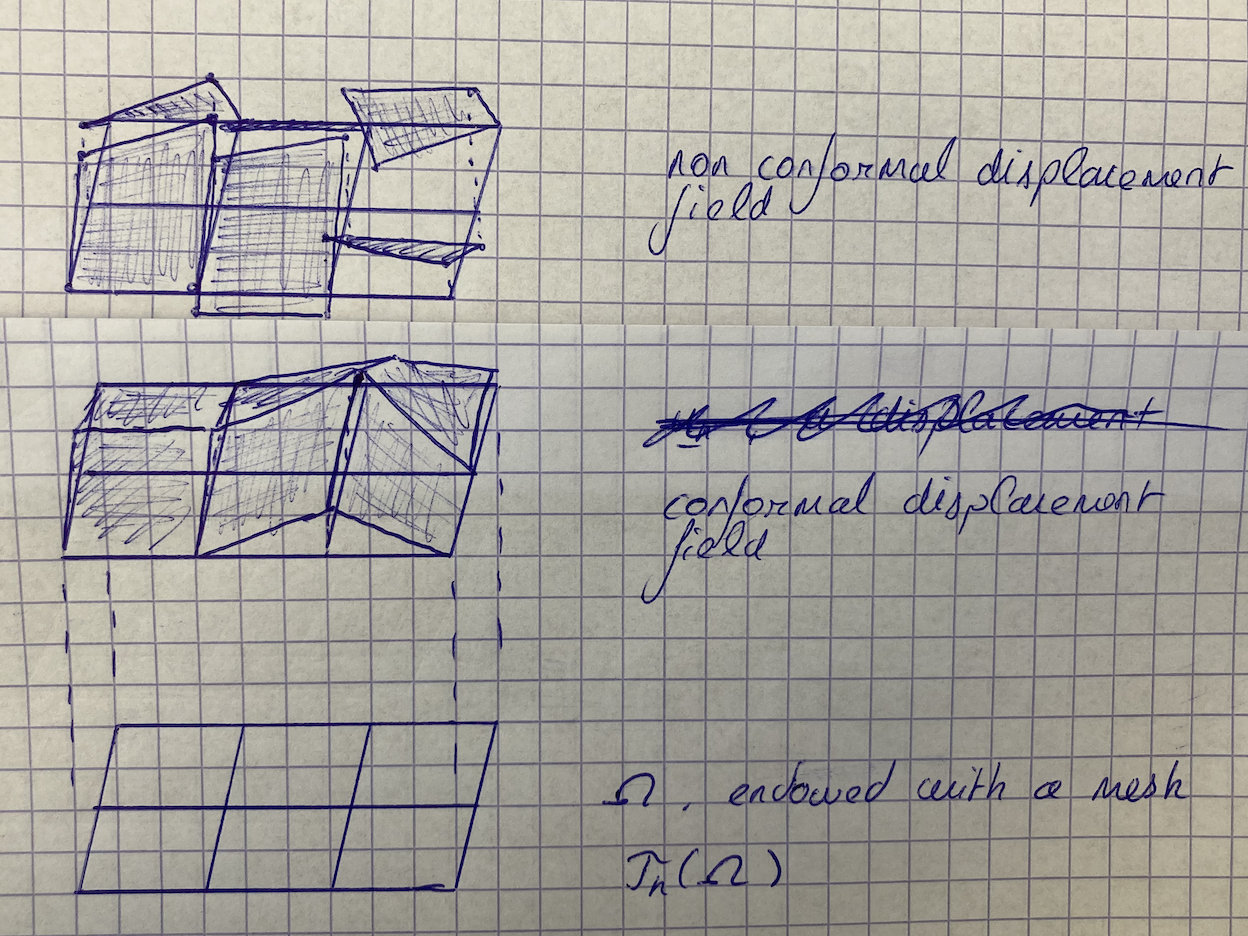
\includegraphics[width=10.cm]{img/discontinuous_displacement.png}
                \caption{Exemples of admissible displacement fields for the Galerkin method (down) and for non-conformal methods (up)}
                \label{fig_discontinuous_displacement}
            \end{figure}

            From a mechnaical standpoint, considering discontinuous displacement amounts to consider matter as a piece-wise continuous medium (as if the body $\Omega$ was made of patches of matter, where each patch corresponds to an element of the triangulation), which is not a physically consistent point of view.
            \newline
            Indeed, if $\Omega$ is a collection of patches of matter that nothing binds together, any patch of matter is free to "debound" and to behave independently. Such a scenario is not envisageable, because any patch would then be free to move from its neighbours up to a rigid body motion. The computational consequence of such a behjavior is that an infinity of admissible displacement fields minimizing the energy in $\Omega$ are possible, which amounts to state that the porblem is ill-posed.

            Hence, an "intermediate" behavior must be considered to bind all patches of matter together and restore a form of continuity in $\Omega$. The natural process would be to striclty force continuity of the displacement at the interface between patches of matter, which would amount to recover the continuous case, and so the Galerkin method. However, another approach can be considered : one can influence continuity of matter in a weaker sense than by forcing it \textit{per se}.
            \newline
            A straightforward way would be to impose a traction force at the interface between patches of matter. The most simple case is to consider an elastic behavior, which can be reprensented by an elastic interphace between elements, that pulls on elements through a traction (or bounding) force. In order to do so, one introduces a support for this interface, namely the skeleton of the mesh $\Mesh(\Omega)$ : it is the collection of all interfaces between two elements, or between an element and the boundary $\partial \Omega$ (see \figref{bones}).
            \newline
            In the same way that bones form the skeleton of the human body, the skeleton of the mesh forms the "structure" of the solid $\Omega$. The collection of patches of matter in $\Omega$ can be seen as the muscular tissue : each muscle is \textit{a priori} free to move with respect to other muscles, but connections exists bteween muscles,
            % and moving the tricep has a consequence on the contraction of the bicep,
            as muscles are linked to bones via sinews. It is the same for the considered setting in $\Omega$ : an intermediate elastic behavior between elements, that plays the role of sinews in the human body, ensures communication of individual patches of matter through the skeleton of the mesh.

            \begin{figure}[h]
                \centering
                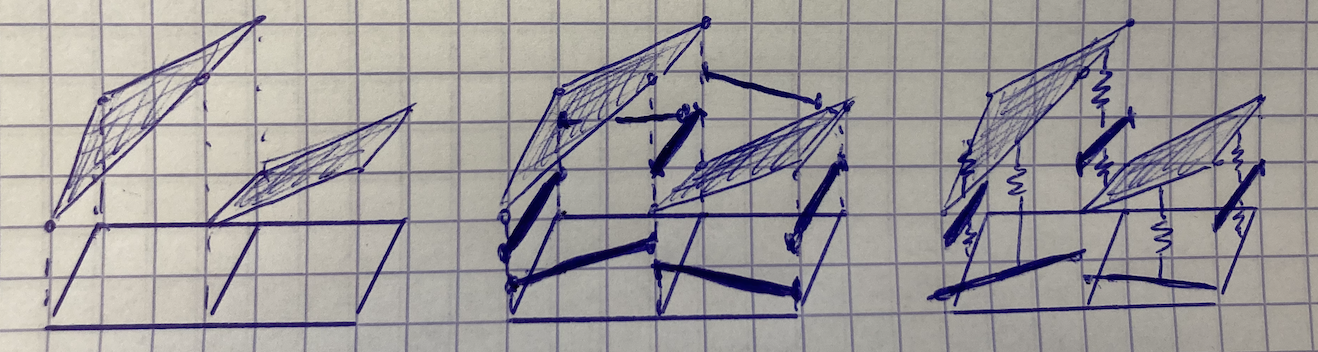
\includegraphics[width=10.cm]{img/bones.png}
                \caption{Introducing the skeleton of $\Mesh(\Omega)$ and bounding forces between patches of matter}
                \label{bones}
            \end{figure}

            \begin{figure}[h]
                \centering
                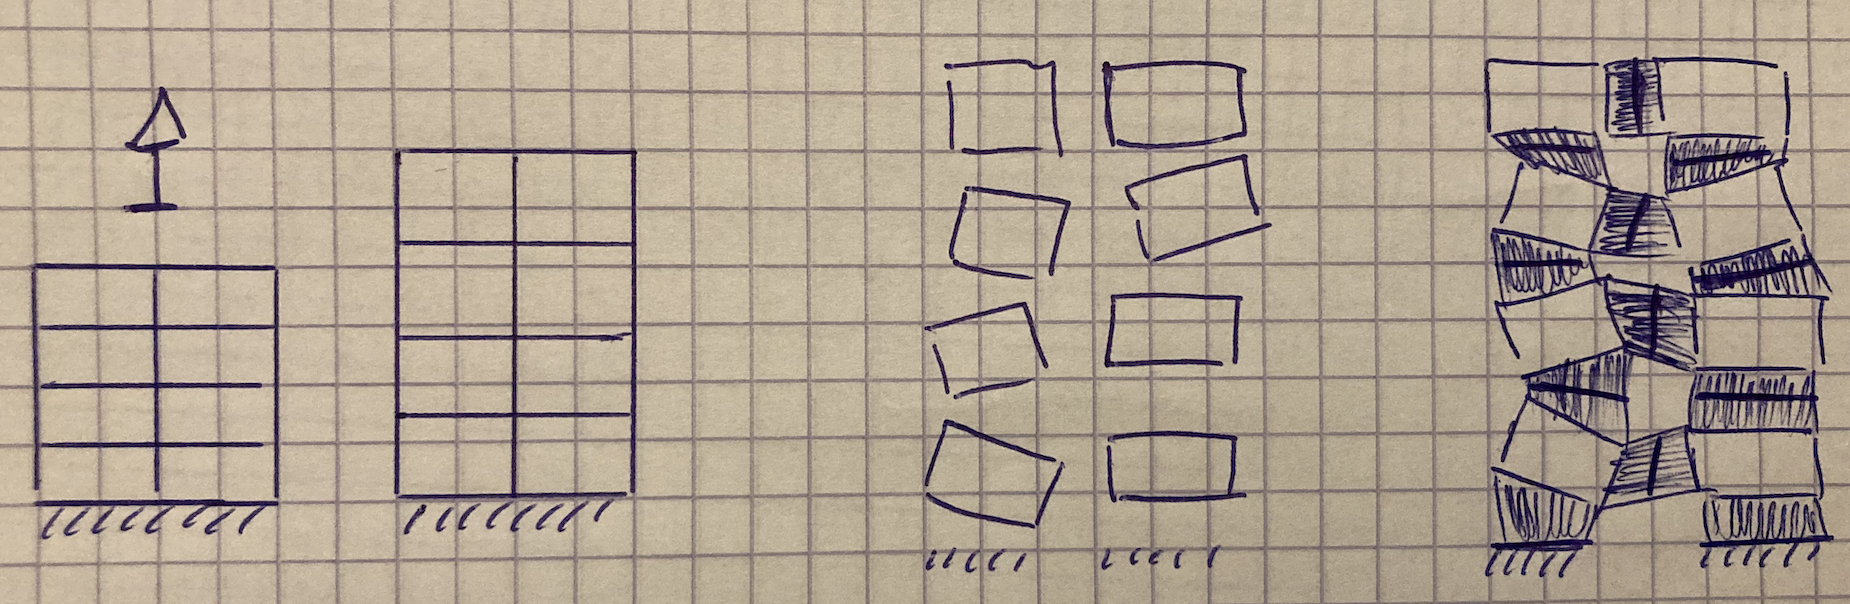
\includegraphics[width=10.cm]{img/deconstruction.png}
                \caption{Illustration of a transition from of the FE representation to a HHO representation}
                \label{fig_setting}
            \end{figure}

        \subsection{Inner traction force, weak continuity and stabilization}
        \label{sec_stabilization}

            Let now specify the formulation of such a traction force between patches of matter. Let consider an element $T \subset \mathbb{R}^d$, atached to a bone (or face) $F \subset \mathbb{R}^{d-1}$ by an elastic membrane $\Gamma \subset \mathbb{R}^d$.

            Let suppose $F$ to be planar (or a point when $d = 1$). The face $F$ has a normal vector $\lighttensori{n}\subscript{F}$ in $\mathbb{R}^d$, such that its sign is arbitrary set so it is outward oriented. Hence, the sign of $\lighttensori{n}\subscript{F}$ changes depending on the considered element.

            \begin{figure}[h]
                \centering
                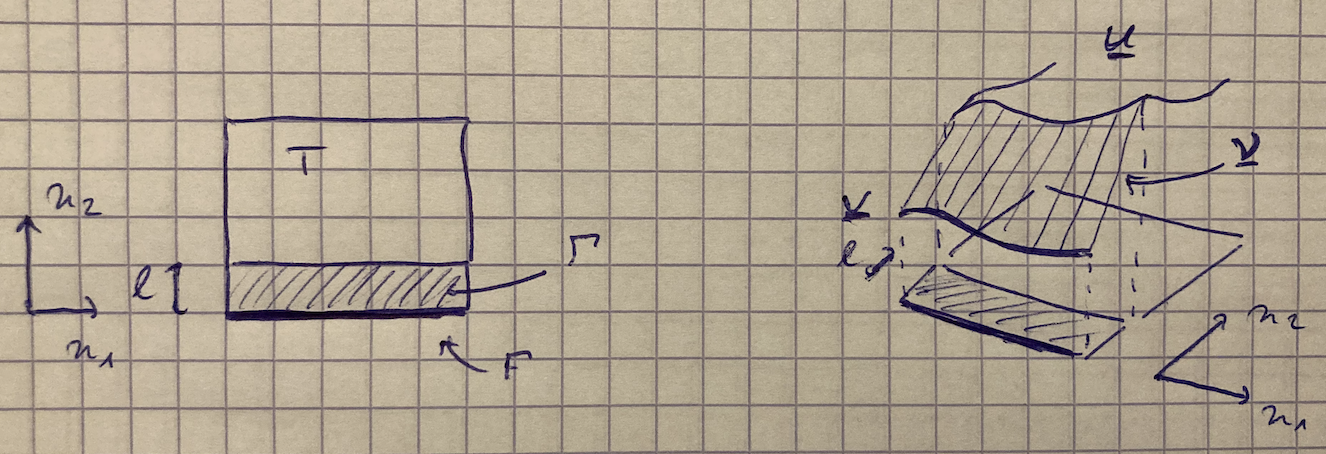
\includegraphics[width=10.cm]{img/setting.png}
                \caption{The considered setting}
                \label{fig_setting}
            \end{figure}

            Let $\mathcal{R}_F = (\lighttensori{x}\subscript{1}, ..., \lighttensori{x}\subscript{d-1}, \lighttensori{x}\subscript{d} = \lighttensori{n}\subscript{F})$ the reference frame in $\mathbb{R}^d$, and let the origin $\lighttensori{0}$ of $\mathcal{R}_F$ in $F$.
            $\Gamma$ is the extrusion of $F$ towards $-\lighttensori{n}\subscript{F}$ by a small depth $l$, such that the volume occupied by $\Gamma$ is $F \cdot l$

            Let consider $\tensori{u}\subscript{\bm{T}}$ a displacement field in $T$, and $\tensori{u}\subscript{\bm{F}}$ a displacement field in $F$. If $l=0$ (\textit{i.e.} if $\Gamma = \emptyset$), the setting conrresponds to that discribed in section \ref{sec_HHO_intro}, where a discontinuous displacement field over $T$ is considered.
            However, considering $l \neq 0$, and setting $\tensori{\nu}\subscript{\bm{\Gamma}}$ the displacement field in $\Gamma$ such that it bridges $\tensori{u}\subscript{\bm{T}}$ to $\tensori{u}\subscript{\bm{F}}$ through $\Gamma$, one recovers the continuous case.

            Let consider the volume $\Gamma \cup T$ made out of a given material with equivalent Young modulus $\beta$, and let suppose that boundary conditions are given in $\partial(\Gamma \cup T)$, in the same way that boundary conditions are given for each element in the FE method. The trick to obtain the expression of a traction force acting on $T$ when $T$ is disconected from $F$, as suggested in \ref{sec_HHO_intro}, consists in expressing the equilibrium in $\partial(\Gamma \cup T)$ and make $l \rightarrow 0$ to meet the discontinuous case.
            In order to do so, let suppose the following hypothesis :

            \paragraph{The interface $\Gamma$ is thin with regards to $T$}
            Let suppose $l$ small in comparison with other dimensions of the problem. Since $l$ is small, let
            linearize $\tensori{\nu}\subscript{\bm{\Gamma}}$ at the first order, such that it bridges $\tensori{u}\subscript{\bm{T}}$ to $\tensori{u}\subscript{\bm{F}}$ :
            \begin{equation}
                \tensori{\nu}\subscript{\bm{\Gamma}}(\lighttensori{x}) = \llbracket \tensori{u} \rrbracket \cdot \frac{x_d}{l} + \tensori{u}\subscript{\bm{F}}
                % \mbox{ with }
                % \llbracket \tensori{u} \rrbracket = (\tensori{u} - \tensori{u})\vert_{T \cap \Gamma}
                % \mbox{ the displacement jump between $F$ and $T$, independent of $x_d$}
            \end{equation}
            with $\llbracket \tensori{u} \rrbracket = \tensori{u}\subscript{\bm{T}}\vert_{T \cap\Gamma} - \tensori{u}\subscript{\bm{F}}
            \mbox{ the displacement jump between $F$ and $T$, independent of $x_d$}$

            \paragraph{The interface $\Gamma$ behaves like a $d-1$ domain}
            Let suppose that $\Gamma$ behaves like a shell when $d = 3$, a beam when $d = 2$ and a point when $d = 1$. Hence, one can write the stress tensor $\tensorii{\sigma} \vert_{\Gamma}$ directly as a traction vector, with a normal component and tangential components. Consequently, the deformation tensor also writes as a vector with same notations.
            \newline
            Moreover, the tractions and deformations on $\Gamma$ are only supposed to depend on the position along the normal component, \textit{i.e.} on $x_d$.
            \newline
            In particular, given the linearized expression of $\tensori{\nu}\subscript{\bm{\Gamma}}$, one has the following deformations and stresses :
            \begin{equation}
                \tensori{\varepsilon}\vert_{\Gamma} = \frac{\llbracket \tensori{u} \rrbracket}{l}
                \mbox{ and }
                \tensori{\sigma}\vert_{\Gamma} = \beta \tensori{\varepsilon}\vert_{\Gamma} = \beta \frac{\llbracket \tensori{u} \rrbracket}{l}
            \end{equation}

            Writing the volumetric contribution of the PVW in $\Gamma \cup T$ yields, $\forall \hat{\tensori{u}}\subscript{\bm{T}}, \hat{\tensori{u}}\subscript{\bm{F}}$ kinematically admissible :
            \begin{equation}
                \label{PVW_1}
                \int_T \tensorii{\sigma} : \nabla \hat{\tensori{u}}\subscript{\bm{T}} + \int_\Gamma \tensori{\sigma} \vert_{\Gamma} \cdot \llbracket \hat{\tensori{u}} \rrbracket
                % = \int_{\partial(\Gamma \cup T)} \tensori{t} \cdot \hat{\tensori{u}}
            \end{equation}
            \begin{equation}
                \int_T \tensorii{\sigma} : \nabla \hat{\tensori{u}}\subscript{\bm{T}} + \int_F \int_{x_d = 0}^{x_d = l} \beta \frac{1}{l} \llbracket \tensori{u} \rrbracket \cdot \llbracket \hat{\tensori{u}} \rrbracket
            \end{equation}
            \begin{equation}
                \int_T \tensorii{\sigma} : \nabla \hat{\tensori{u}}\subscript{\bm{T}} + \int_F \beta \llbracket \tensori{u} \rrbracket \cdot \llbracket \hat{\tensori{u}} \rrbracket
            \end{equation}

            Hence, the traction force of $F$ onto $T$ is $\displaystyle \tensori{T}\subscript{F \rightarrow T} = \int_F \beta \llbracket \tensori{u} \rrbracket$.

            \begin{figure}[h]
                \centering
                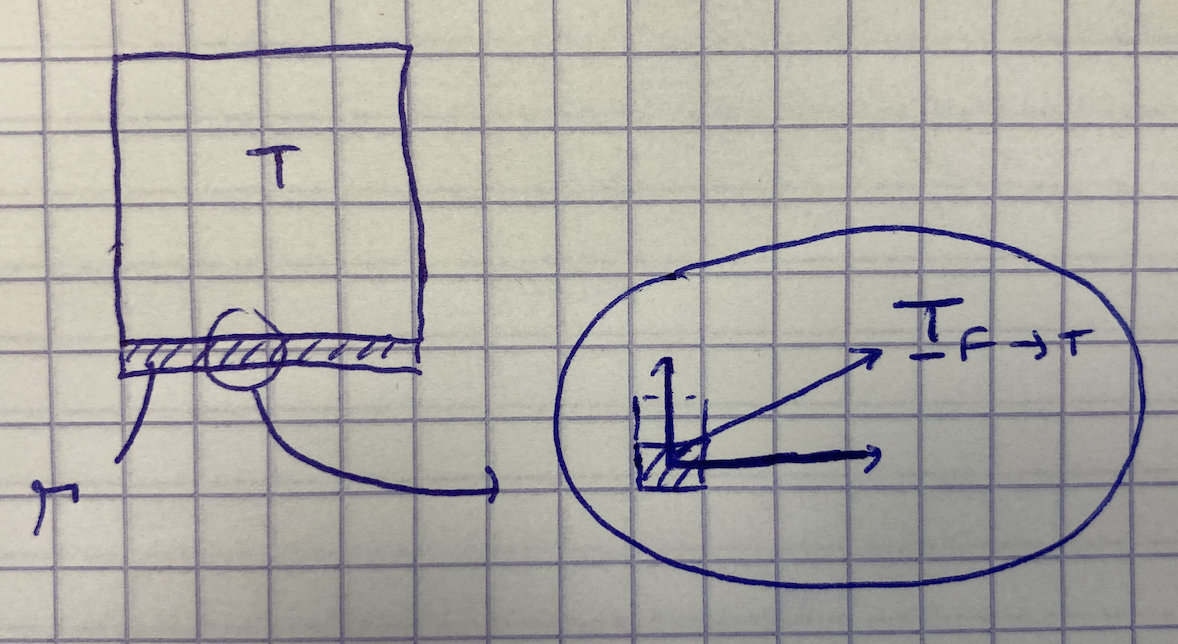
\includegraphics[width=10.cm]{img/traction.png}
                \caption{Illustration of the traction vector in a portion of $\Gamma$ acting on $T$}
                \label{fig_traction}
            \end{figure}
            
            Making $l \rightarrow 0$ allows to recover the discontinuous case where the skeleton of the mesh is actually of dimension $d-1$, and generalizing the previous argument to all faces in $\partial T$ yields the following PVW in the discontinuous case :

            \begin{equation}
                \begin{aligned}
                    &
                    \int_T \tensorii{\sigma} : \nabla \hat{\tensori{u}}\subscript{\bm{T}} + \int_{\partial T} \beta \llbracket \tensori{u} \rrbracket \cdot \llbracket \hat{\tensori{u}} \rrbracket
                    =
                    \int_{\partial T} \tensori{t}\subscript{N} \cdot \hat{\tensori{u}}\subscript{\bm{F}}
                    &&
                    \mbox{in $T$}
                    \\
                    &
                    \tensori{u}\subscript{\bm{F}} = \tensori{u}\subscript{D}
                    &&
                    \mbox{on $\partial T$}
                \end{aligned}
            \end{equation}

            From a more mathematical standpoint, the traction force at the interface is a weak form of continuity, through a penalization in the least square sense of the displacement jump at the discontinuity. 

        \subsection{Discrete gradient operator, contnuity and polynomial order of the derivative}

            From a numerical perspective, introducing a skeleton over $\Mesh(\Omega)$ implies to introduce more unknowns, and setting the displacement to be discontinuous suggests the use of a different polynomial basis than the Lagrange one, which is not a bargain.

            The reason for introducing such a setting is that now that elements are endowed with a rigid body motion (though stabilized by the action of the elastic interface), more degrees of freedom are possible in each element. This feature is what allows to reconsider the notion of derivation for the displacement field in $\Mesh(\Omega)$ : instead of the regular gradient operator $\nabla$ (which takes the form of the matrix $\tensorii{\mathbbl{B}}$ in the FE method), an "enriched" gradient operator will be considered, such that it provides the projection of the gradient of the displacement field in the continuous polynomial space.

            Providing an enhanced approximation of the derivative of the displacement field with comparison to that provided by the Galerkin method is the main purpose of non conformal methods.

            Let consider the same setting as in \ref{sec_stabilization}, with an element $T$ and an interface $\Gamma$ linking $T$ to $F$ a face in $\partial T$. With same notations, let $\tensori{u}\subscript{\bm{T}}$ the displacement field in $T$, $\tensori{u}\subscript{\bm{F}}$ that in $F$ and $\tensori{\nu}\subscript{\bm{\Gamma}}$ that in $\Gamma$. Moreover, let suppose $\tensori{u}\subscript{\bm{T}}, \tensori{u}\subscript{\bm{F}}$ and $\tensori{\nu}\subscript{\bm{\Gamma}}$ polynomials of given order $k$ ; hence, their derivatives  are polynomials of order $k-1$.

            In $T \cap \Gamma$, one has the continuous displacement field :
            \begin{equation}
                \tensori{u}\subscript{\bm{T \cup \Gamma}}(\lighttensori{x}) = 
                \begin{cases}
                    \tensori{u}\subscript{\bm{T}}(\lighttensori{x}) & \mbox{if } \lighttensori{x} \in T
                    \\
                    \tensori{\nu}\subscript{\bm{\Gamma}}(\lighttensori{x}) & \mbox{if } \lighttensori{x} \in \Gamma
                \end{cases}
            \end{equation}

            Let suppose the displacement field in $T \cup \Gamma$ the Galerkin approximation of the solution for a given problem : $\tensori{u}\subscript{\bm{T \cup \Gamma}}$ is then the projection of the exact solution $\tensori{u}$ onto the space of continuous polynomials of order $k$ in $\Omega$. Writing $\tensori{w}\subscript{\bm{\perp}}$ the orthogonal of $\tensori{u}\subscript{\bm{T \cup \Gamma}}$ in the complementary space to that of continuous polynomials of order $k$ in $\Omega$, one can write :
            \begin{equation}
                \tensori{u} = \tensori{u}\subscript{\bm{T \cup \Gamma}} + \tensori{w}\subscript{\bm{\perp}}
            \end{equation}
            And taking its gradient yields :
            \begin{equation}
                \nabla \tensori{u} = \nabla \tensori{u}\subscript{\bm{T \cup \Gamma}} + \nabla \tensori{w}\subscript{\bm{\perp}}
            \end{equation}
            For all $\tensorii{\tau}$ polynomial-valued tensor of order $k$ :
            \begin{equation}
                \begin{aligned}
                    \int_{T \cup \Gamma} \nabla \tensori{u} : \tensorii{\tau}
                    =
                    \int_{T \cup \Gamma} \nabla \tensori{u}\subscript{\bm{T \cup \Gamma}} : \tensorii{\tau}
                    +
                    \int_{T \cup \Gamma} \nabla \tensori{w}\subscript{\bm{\perp}} : \tensorii{\tau}
                \end{aligned}
            \end{equation}
            Which gives after applying the divergence theorem :
            \begin{equation}
                \label{eq_gradient_0}
                \begin{aligned}
                    \int_{T \cup \Gamma} \nabla \tensori{u} : \tensorii{\tau}
                    =
                    \int_{T \cup \Gamma} \nabla \tensori{u}\subscript{\bm{T \cup \Gamma}} : \tensorii{\tau}
                    +
                    \int_{T \cup \Gamma} \tensori{w}\subscript{\bm{\perp}} \cdot (\nabla \cdot \tensorii{\tau})
                    +
                    \int_{F} \tensori{w}\subscript{\bm{\perp}} \cdot (\tensorii{\tau} \ \lighttensori{n}\subscript{F})
                \end{aligned}
            \end{equation}
            Since $\tensori{w}\subscript{\bm{\perp}}$ is orthogonal to the displacement approximation space, its projection onto it is zero. Moreover, $\forall \tensorii{\tau}, \nabla \cdot \tensorii{\tau}$ is in the displacement approximation space as a polynomial of order $k-1$. Thus :
            \begin{equation}
                \int_{T \cup \Gamma} \tensori{w}\subscript{\bm{\perp}} \cdot (\nabla \cdot \tensorii{\tau}) = 0
            \end{equation}
            And \eqref{eq_gradient_0} becomes :
            \begin{equation}
                \begin{aligned}
                    \label{eq_gradient_1}
                    \int_{T \cup \Gamma} \nabla \tensori{u} : \tensorii{\tau}
                    =
                    \int_{T \cup \Gamma} \nabla \tensori{u}\subscript{\bm{T \cup \Gamma}} : \tensorii{\tau}
                    +
                    \int_{F} \tensori{w}\subscript{\bm{\perp}} \cdot (\tensorii{\tau} \ \lighttensori{n}\subscript{F})
                \end{aligned}
            \end{equation}



  \end{document}